% fig_crosspol_timing.tex
% TR-30: Timeline showing memory hold vs zone timers for 3PH and non-3PH faults
%
% X range: 0 to 14 cm ≡ 0 to 650 ms  (scale: 14/650)
% Memory hold: 0–100 ms ≡ 0–2.154 cm
% Zone 1: 20 ms ≡ 0.431 cm
% Zone 2: 300 ms ≡ 6.462 cm
% Zone 3: 600 ms ≡ 12.923 cm
%
% Precomputed (to avoid pgfmathsetmacro name clashes):
%   xZ1  = 20/650*14  = 0.431
%   xMem = 100/650*14 = 2.154
%   xZ2  = 300/650*14 = 6.462
%   xZ3  = 600/650*14 = 12.923
%   xEnd = 14.0

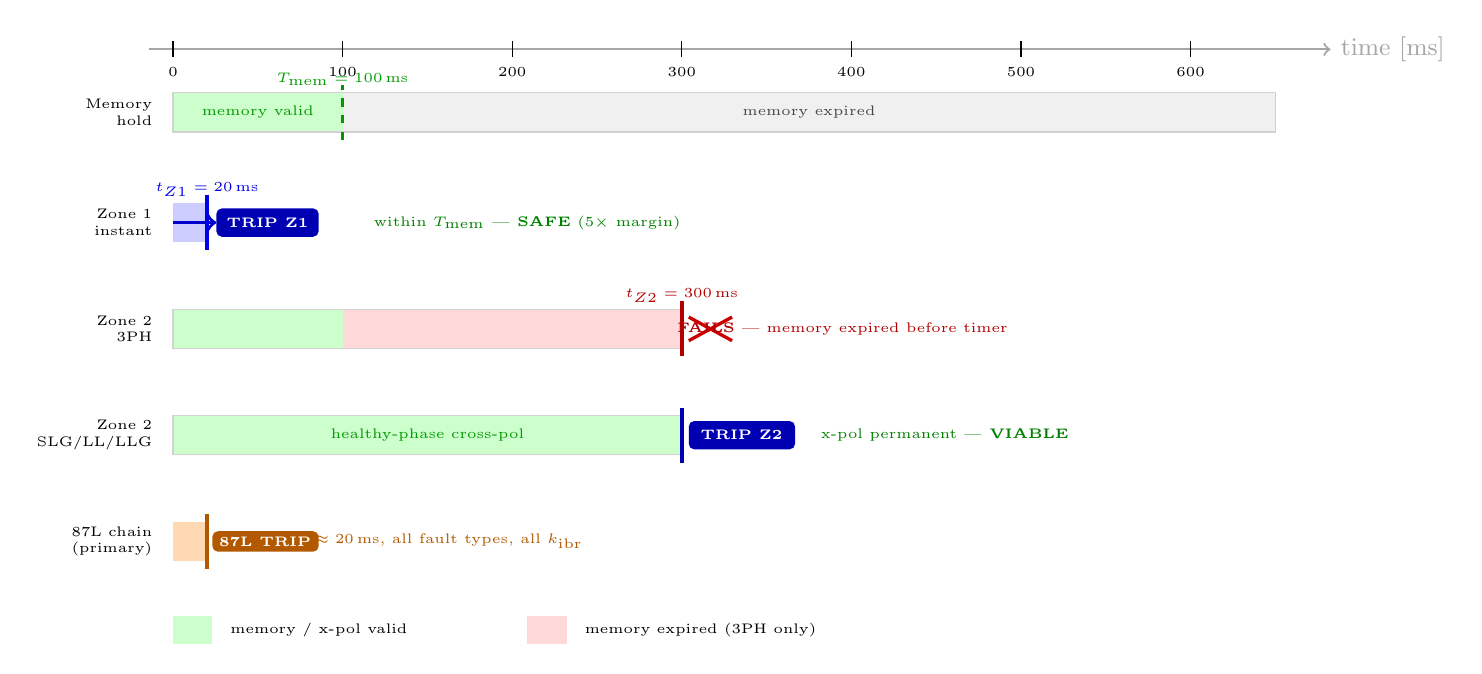
\begin{tikzpicture}[
  every node/.style = {font=\scriptsize},
]

% ── X-axis ──────────────────────────────────────────────────────────────────
\draw[->, thick, gray!70] (-0.3, 0) -- (14.7, 0)
  node[right, font=\small] {time [ms]};

\foreach \tmk/\xloc in {0/0, 100/2.154, 200/4.308, 300/6.462, 400/8.615, 500/10.769, 600/12.923} {
  \draw (\xloc, -0.10) -- (\xloc, 0.10);
  \node[below=3pt, font=\tiny] at (\xloc, 0) {\tmk};
}

% ── Row 1: Memory hold region ──────────────────────────────────────────────
\fill[green!20]       (0, -1.05) rectangle (2.154, -0.55);
\fill[gray!12]        (2.154, -1.05) rectangle (14.0, -0.55);
\draw[gray!35]        (0, -1.05) rectangle (14.0, -0.55);
\draw[green!60!black, very thick, dashed] (2.154, -1.15) -- (2.154, -0.45);
\node[green!60!black, font=\tiny] at (1.077, -0.80) {memory valid};
\node[gray!55!black,  font=\tiny] at (8.077, -0.80) {memory expired};
\node[green!60!black, font=\tiny] at (2.154, -0.38) {$T_\mathrm{mem}=100$\,ms};
\node[left=4pt, align=right, font=\tiny] at (0, -0.80) {Memory\\hold};

% ── Row 2: Zone 1 (always safe) ─────────────────────────────────────────────
\fill[blue!20]   (0, -2.45) rectangle (0.431, -1.95);
\draw[blue!80!black, very thick, ->] (0, -2.20) -- (0.55, -2.20);
\draw[blue!90!black, very thick] (0.431, -2.55) -- (0.431, -1.85);
\node[blue!90!black, font=\tiny] at (0.431, -1.78) {$t_{Z1}=20$\,ms};
\fill[blue!70!black, rounded corners=2pt]
  (0.55, -2.38) rectangle (1.85, -2.02);
\node[white, font=\tiny] at (1.20, -2.20) {\textbf{TRIP Z1}};
\node[green!50!black, font=\tiny] at (4.5, -2.20)
  {within $T_\mathrm{mem}$ --- \textbf{SAFE} ($5\times$ margin)};
\node[left=4pt, align=right, font=\tiny] at (0, -2.20) {Zone~1\\instant};

% ── Row 3: Zone 2 — 3PH fault (fails) ──────────────────────────────────────
\fill[green!20]       (0, -3.80) rectangle (2.154, -3.30);
\fill[red!15]         (2.154, -3.80) rectangle (6.462, -3.30);
\draw[gray!35]        (0, -3.80) rectangle (6.462, -3.30);
\draw[red!70!black, very thick] (6.462, -3.90) -- (6.462, -3.20);
\node[red!70!black, font=\tiny] at (6.462, -3.13) {$t_{Z2}=300$\,ms};
% X mark (no trip)
\draw[red!80!black, very thick] (6.55, -3.70) -- (7.10, -3.40);
\draw[red!80!black, very thick] (6.55, -3.40) -- (7.10, -3.70);
\node[red!70!black, font=\tiny] at (8.5, -3.55)
  {\textbf{FAILS} --- memory expired before timer};
\node[left=4pt, align=right, font=\tiny] at (0, -3.55) {Zone~2\\3PH};

% ── Row 4: Zone 2 — SLG/LL/LLG (viable) ────────────────────────────────────
\fill[green!20]   (0, -5.15) rectangle (6.462, -4.65);
\draw[gray!35]    (0, -5.15) rectangle (6.462, -4.65);
\draw[blue!70!black, very thick] (6.462, -5.25) -- (6.462, -4.55);
\fill[blue!70!black, rounded corners=2pt]
  (6.55, -5.08) rectangle (7.90, -4.72);
\node[white, font=\tiny] at (7.22, -4.90) {\textbf{TRIP Z2}};
\node[green!50!black, font=\tiny] at (9.8, -4.90)
  {x-pol permanent --- \textbf{VIABLE}};
\node[green!60!black, font=\tiny] at (3.231, -4.90)
  {healthy-phase cross-pol};
\node[left=4pt, align=right, font=\tiny] at (0, -4.90) {Zone~2\\SLG/LL/LLG};

% ── Row 5: 87L chain (reference) ────────────────────────────────────────────
\fill[orange!30]  (0, -6.50) rectangle (0.431, -6.00);
\draw[orange!70!black, very thick] (0.431, -6.60) -- (0.431, -5.90);
\fill[orange!70!black, rounded corners=2pt]
  (0.50, -6.38) rectangle (1.85, -6.12);
\node[white, font=\tiny] at (1.17, -6.25) {\textbf{87L TRIP}};
\node[orange!70!black, font=\tiny] at (3.5, -6.25)
  {$\approx20$\,ms, all fault types, all $k_\mathrm{ibr}$};
\node[left=4pt, align=right, font=\tiny] at (0, -6.25) {87L chain\\(primary)};

% ── Legend ──────────────────────────────────────────────────────────────────
\fill[green!20]  (0.0, -7.55) rectangle (0.50, -7.20);
\node[right=3pt, font=\tiny] at (0.50, -7.37) {memory / x-pol valid};
\fill[red!15]    (4.5, -7.55) rectangle (5.0, -7.20);
\node[right=3pt, font=\tiny] at (5.0, -7.37) {memory expired (3PH only)};

\end{tikzpicture}
